% Template for ICASSP-2018 paper; to be used with:
%          spconf.sty  - ICASSP/ICIP LaTeX style file, and
%          IEEEbib.bst - IEEE bibliography style file.
% --------------------------------------------------------------------------
\documentclass{article}
\usepackage{spconf,amsmath,graphicx}
\graphicspath{{images/}}

% Example definitions.
% --------------------
% \def\x{{\mathbf x}}
% \def\L{{\cal L}}

\title{Neural Speech-To-Speech Synthesis}
\name{Jared Samet - UNI: jss2272}
\address{jss2272@columbia.edu}
\begin{document}
%\ninept
%
\maketitle
%
\begin{abstract}
  Prosody features that transfer across speakers can be extracted using unsupervised learning. By adding the cluster labels as annotation to text, a text-to-speech synthesis system can learn to incorporate the prosody into its output. The resulting system can produce audio that is different even when the text is the same and the resulting audio can mimic the prosody from the original speaker. The abstract should be about 175 words total.
\end{abstract}
%
\begin{keywords}
Prosody, unsupervised learning, speech synthesis, seq2seq
\end{keywords}
%
\section{Introduction}
\label{sec:intro}

I used Kaldi \cite{Povey_ASRU2011} to create an alignment for the Tedlium data using the final triphone model it created. For each vowel phoneme, I used Kaldi's pitch extractor and the first MFCC component (energy) to create two series of numbers. Kaldi's pitch extractor is already normalized but I used [StandardScaler] to normalize the energy component across the utterance. I fit a second-degree (?) Legendre polynomial to the pitch and power to create six features for each vowel. The duration gave me the seventh feature. I then ran K-means clustering on these to create eight different vowel clusters that were common across the entire range of speakers in the (subsampled) Tedlium data.

I then used the same triphone model to generate an alignment for the LJSpeech dataset, extracted the same pitch, power, and duration features for LJ, and used the previously computed vowel clusters to assign a cluster label to each vowel in the LJSpeech dataset. I (slightly) modified the Tacotron implementation to accept a sequence of tokens instead of a sequence of characters. Instead of text characters, my input tokens consisted of (Kaldi's) phonemes and the vowel cluster labels. Having suitably modified Tacotron, I then trained Tacotron on the [phoneme + cluster label, audio] pairs.

Finally, to see if it worked, I recorded myself saying a sentence in multiple ways, ran each .wav through the same align + label steps, and fed the resulting [phoneme+label, text] pairs to Tacotron. She said the same thing different ways.

\section{Related Work}
\label{sec:sota}

This project involved two main components: first, extracting prosody features from a set of input audio files; and second, training a text-to-speech synthesis model on a dataset that had been labeled using the extracted prosody features.

Selkirk \cite{selkirk1995sentence} discusses sentence prosody and pitch accent in the context of English. Although English is generally not thought of as a tonal language, Selkirk writes that ``[i]n English a pitch accent associates to a stress-prominent syllable in a word (typically the main word stress.)''
Ghahremani et al. \cite{ghahremani2014pitch} describes an pitch-extraction algorithm (``the Kaldi pitch tracker'') based on Talkin \cite{talkin1995robust} that is specifically designed for use in the speech recognition concept and is implemented in the open-source Kaldi project \cite{}. This project uses that implementation to extract the pitch contour.
Fujisaki \cite{fujisaki2004information} models the $F_0$ contour over the duration of an utterance as the sum of a set of impulse response and step response functions, parameterized with a finite number of scalar values.
Wang et al. \cite{wang2008mandarin} use the pitch and amplitude contours to improve tone recognition in Mandarin by identifying ``maxima, minima, and inflection points of particular acoustic events.''
Wong and Siu \cite{pui2004decision} use robust regression and orthogonal polynomials to create features for a decision tree classifier in order to recognize tones in Chinese lan guages. Finally, Lin \cite{lin2005language} and Mary \cite{mary2011extraction} use a small number of Legendre polynomial coefficients to represent the pitch contour as a finite-dimensional feature vector, which is the approach used in this project.

Speech synthesis or text-to-speech is a well-studied problem that has been actively researched since the 1950s. While there has been remarkable progress in the field in recent years, the quality of computer-generated speech has not yet reached human levels. Current commercial systems described in Khan et al. \cite{khan2016concatenative} and Taylor  \cite{taylor2009text} generally use concatenative speech synthesis to produce their output. However, the alternative approach of parametric synthesis using neural networks is rapidly gaining popularity, with several papers since 2016 demonstrating impressive results in the quality of the output.
The first of this generation was Google's WaveNet (Oord et al. \cite{oord2016wavenet}), followed in quick succession by Deep Voice and Deep Voice 2 from Baidu (Arik et al. \cite{arik2017deep}, \cite{arik2017deep2}), Char2Wav from MILA (Sotelo et al. \cite{sotelo2017char2wav}), and Tacotron from Google (Wang et al. \cite{wang2017tacotron}).
Each of these systems has taken a different approach to the network architecture to address different aspects of the speech synthesis pipeline. Tacotron, which is the backend used in this project, is an end-to-end text-to-speech system based on the sequence-to-sequence with attention model. As the authors describe, ``The model takes characters as input and outputs the corresponding raw spectrogram, which is then fed to the Griffin-Lim reconstruction algorithm to synthesize speech.''

\section{Overview}
\label{sec:overview}
The goal of this project was to create a system that, given an input audio file from an arbitrary speaker, produces a synthesized audio output of the same utterance in the voice of a second speaker, where the prosody of the output audio matches that of the input audio as closely as possible.
The system implemented uses a pipeline of several processing steps in order to accomplish this.
An overview of the pipeline and a diagram are presented here for context; a detailed description of each step follows.

The first portion of the system is the vowel-cluster training process, which takes as input a previously-trained acoustic model for alignment and a speech dataset from multiple speakers. As output, it produces a clustering model that can be used to annotate an audio utterance from an arbitrary speaker with cluster labels for each vowel in the utterance. This portion of the system uses Kaldi to, first, perform forced alignment on the multi-speaker dataset, and, second, to extract the pitch contour and the first (energy) MFCC component for each frame of the input audio. Given the alignment, pitch, and power contours, an unsupervised clustering algorithm (K-means) trained on the audio segments corresponding to vowels to learn several distinct ways in which syllables can be pronounced.

The second portion of the system is the speech-synthesis training process, which takes as input the pre-existing acoustic model, the newly-trained vowel-cluster model, and a large speech dataset from a single speaker. As output, it produces a trained Tacotron model that can be used to generate synthesized utterances. This portion of the system first uses Kaldi to perform forced alignment on the speech dataset and extract the pitch and power features, as before. It then uses the vowel-cluster model to produce an annotated phoneme sequence for each utterance in the single-speaker dataset. Finally, the audio and the annotated phoneme sequence pairs are used to train the Tacotron model.

The final portion of the system is generates new utterances. As input, it takes the pre-existing acoustic model, the newly-trained vowel-cluster model, and the newly-trained Tacotron model, and an input audio file in the voice of an arbitrary speaker. As output, it produces synthesized audio of the equivalent utterance where the prosody matches that of the input utterance as closely as possible. This portion of the system computes an alignment for the input utterance and extracts the pitch and power features; uses the vowel cluster model to produce an annotated phoneme sequence for the input utterance; and, finally, uses the newly-trained Tacotron model to synthesize the output audio.

\begin{figure}[htb]

\begin{minipage}[b]{1.0\linewidth}
  \centering
  \centerline{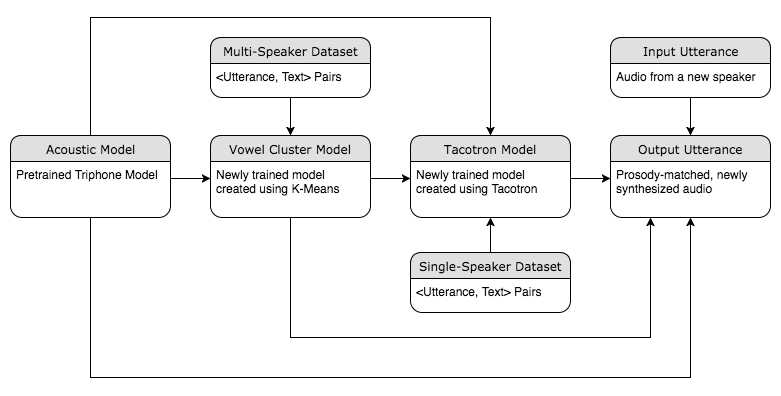
\includegraphics[width=8.5cm]{Overall_Pipeline}}
\end{minipage}
\caption{Pipeline Overview}
\label{fig:overview}
\end{figure}

\section{Prosody Feature Extraction}
\label{sec:prosody}

All three portions of the pipeline involve extracting prosody features from the input audio -- in the vowel-cluster training process, the input audio is the multi-speaker dataset; in the single-speaker annotation process, the input audio is the single-speaker dataset; and in the utterance-generation portion, the input audio is the new utterance the user wishes to re-synthesize in a new voice.
The prosody feature extraction is performed in three steps; Figure \ref{fig:prosodyextraction} shows a diagram.

First, Kaldi's \texttt{align.sh} script uses a pretrained acoustic triphone model -- in this project, the final triphone model resulting from Kaldi's TEDLIUM recipe -- to compute a forced alignment of the input audio, and Kaldi's \texttt{ali-to-phones} tool is used to convert the model-level alignment to a sequence of \textit{(phone\_id, start\_time, end\_time)} tuples.
Next, Kaldi's \texttt{make\_mfcc\_pitch.sh} script creates the MFCC and pitch features for each frame of the input audio, the \texttt{copy-matrix} tool converts this to a text file, and my python script \texttt{kaldi\_to\_npz.py} converts the text file to a numpy array (.npz) file.
Finally, seven real-valued features are created for each vowel phone in the alignment.

The first three features are the coefficients of the second-degree Legendre series that is the least-squares fit to a series of $(x, y)$ points where the length of the series is the computed number of frames plus 4, the $x$ values are evenly spaced between -1 and 1, and the $y$ values are the frame-by-frame pitch values computed using Kaldi's pitch-extraction algorithm, starting two frames before the beginning of the phone and ending two frames after the end of the phone.
Since Kaldi's algorithm already normalizes the pitch contour over a three-second window, no further normalization is done before computing the Legendre coefficients.

The next three features are the Legendre coefficients for the power (first MFCC component) component, calculated in the same way as for the pitch features. Since this component is not normalized by Kaldi, my system normalized the coefficient to have mean zero and unit variance over the whole utterance before computing these coefficients.
The seventh feature is simply the duration of the phone.

These seven features were chosen in the hopes of maximizing the useful prosodic information available in a small set of numbers per phoneme.
The two frames (20 ms) before and after the utterance are added to the sequence to improve the conditioning of the least-squares fit matrix; to compensate for potential slight errors in the alignment as computed by Kaldi; and to provide a small degree of context for the vowel in question.
The domain is fixed at [-1, 1] so that the coefficients capture the level, slope and curvature over the length of the phoneme, regardless of the duration.
Due to the structure of the Legendre polynomials, the three features for the pitch and power series contain information about whether the vowel is pronounced with a rising, falling, or flat tone, and whether the vowel contained a local maximum or minimum of pitch or power.
Finally, the duration feature is a simple attempt to detect whether the vowel is pronounced quickly or is drawn-out.

Most importantly, these features are intended to be useful for identifying which syllables in an utterance are stressed. As Selkirk \cite{selkirk1995sentence} discusses, ``In English a pitch accent associates to a stress-promiment syllable in a word (typically the main word stress).''
However, spoken English uses pitch contour to convey more information than simply which syllable is a word is stressed. Pierrehumbert \cite{pierrehumbert1980phonology} identifies 22 different patterns that an English phrase can exhibit, consisting of various combinations of pitch accent, phrase accent, and intonation occurring at the end of a phrase.
These phrases carry semantic content beyond the actual words of the text. For example, different stress patterns can indicate surprise, emphasis, disbelief, or neutrality, among others.

Figure \ref{fig:pitchpow1} displays the pitch and power contours that Kaldi computes for two pronunciations of the the two-word phrase ``another orange'' (the phrase is from Pierrehumbert \cite{pierrehumbert1980phonology}.) In the first audio file, the words are spoken with a neutral tone. In the second pronunciation, the words are spoken with a tone of disbelief, i.e., ``a\textbf{NOTH}er orange???''. The seven computed features for each vowel are displayed in Table \ref{table:pitchpow1}.

\begin{figure}[htb]

\begin{minipage}[b]{1.0\linewidth}
  \centering
  \centerline{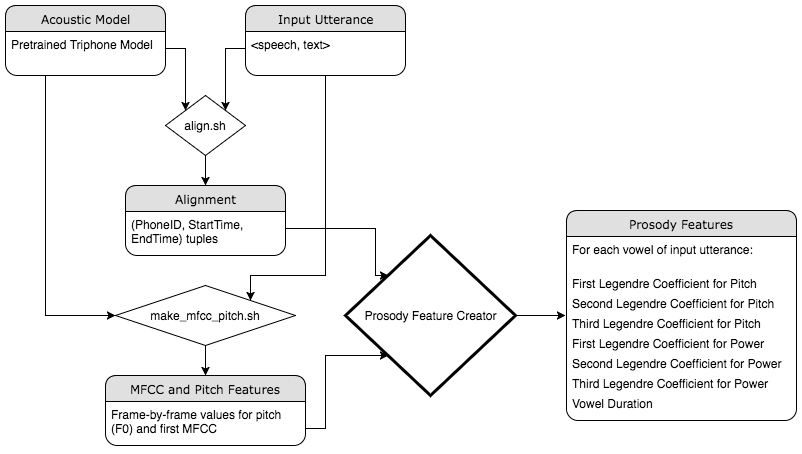
\includegraphics[width=8.5cm]{Prosody_Extraction.png}}
\end{minipage}
\caption{Prosody Feature Extraction}
\label{fig:prosodyextraction}
\end{figure}

\section{Vowel Clustering}
\label{sec:vowels}

To the extent that the seven extracted prosody features for each vowel do indeed convey useful information, there are numerous ways one could imagine using them to ``clone'' an input utterance.
For example, the speech output of a speech synthesis system could be distorted in some smooth way in order to try and match the pitch and power contours of the entire input audio.
Alternately, they could be used as the inputs to a supervised classification algorithm that learned to classify each syllable as stressed or unstressed, with the help of a manually-annotated dataset.
The system I implemented uses $k$-means, an unsupervised algorithm, to partition the space of features into 8 categorical cluster labels.

As stated in Sec. \ref{sec:overview}, the input to the vowel-cluster training process consists of an acoustic model and a multi-speaker speech dataset.
The prosody features for each vowel in the dataset are first computed using the acoustic model as described in Sec. \ref{sec:prosody}.
These features are then normalized over the entire dataset to have zero mean and unit variance on a feature-by-feature basis.
Finally, $k$-means clustering with $k$=8 returns eight vectors in $\mathbf{R}^7$ corresponding to the cluster centroids.
The resulting vowel cluster model therefore consists of the scaling factors that normalize each feature of the input dataset and the eight cluster centroids. This portion of the system was implemented using \texttt{scikit-learn} \cite{scikit-learn}.

There were number of choices involved in how to perform the clustering, including the number of clusters, the use of an unsupervised algorithm as opposed to a supervised algorith, and the decision to use a single set of cluster labels for all vowels, as opposed to computing clusters for each vowel individually. These choices are discussed further in Sec. \ref{sec:discussion}.


Here I need to demonstrate that the clusters are in fact "semantically" different in some way. Maybe include some metric of these or run TSNE on the coefficients.

\section{Speech Synthesis}
\label{sec:tacotron}

The speech-synthesis training portion of the system produces a model that can be used to generate new utterances. The input to this portion of the system is the pretrained acoustic model, the vowel-clustering model resulting from Sec. \ref{sec:vowels}, and a large single-speaker dataset consisting of [text, audio] pairs.
In this phase, the prosody features are first extracted as described in Sec. \ref{sec:prosody}. Next, the vowel-clustering model is used to assign cluster labels to each vowel in the dataset.
The result is a set of [labeled-phone-sequence, audio] pairs; for a single utterance in the dataset, the labeled phone sequence for that utterance is the sequence of phones along with the cluster labels for each vowel. For example, the text for one short utterance in the dataset used here is ``In 1813''.
The corresponding labeled phone sequence is ``IH VOWEL4 N sp SIL EY VOWEL1 T IY VOWEL4 N sp TH ER VOWEL6 T IY VOWEL2 N sp SIL''. The ``sp'' tokens correspond to word boundaries.

The Tacotron \cite{wang2017tacotron} neural network system was trained on the [labeled phone sequence, audio] pairs to produce audio.
Tacotron's internal neural network architecture is far too complex to describe in detail in this paper. As a brief overview, it is based on the Sutskever et al \cite{sutskever2014sequence} encoder-decoder seq2seq model with Bahdanau \cite{bahdanau2014neural} attention. The input is a sequence of one-hot-encoded characters.
The encoder embeds the characters in a continuous vector space, and passes them through the CBHG module described in the Tacotron paper.
The decoder uses GRUs with attention to produce linear-scale spectrogram as the output sequence.

Since Tacotron is agnostic to the character set, I used the phones and the cluster labels, along with the word-boundary marker, as the character set. Tacotron's neural network architecture makes this possible out-of-the-box; it was specifically designed to accomodate end-to-end training using only audio and the corresponding text as its inputs, in contrast to the relatively complex requirements for most speech synthesis systems.
One specific advantage discussed by the authors is that ``it more easily
allows for rich conditioning on various attributes''. The vowel cluster labels used here are an example of this conditioning.

For this project, I used Keith Ito's open-source implementation of Tacotron, with only small modifications required to accomodate my modified character set. The model was trained with his LJ Speech Dataset \cite{ljspeech17}, which he describes on his website as follows:
``This is a public domain speech dataset consisting of 13,100 short audio clips of a single speaker reading passages from 7 non-fiction books. A transcription is provided for each clip. Clips vary in length from 1 to 10 seconds and have a total length of approximately 24 hours. The texts were published between 1884 and 1964, and are in the public domain. The audio was recorded in 2016-17 by the LibriVox project and is also in the public domain.''

The result of this portion of the system is a trained model that takes a labeled phone sequence as input and produces audio as output.

\section{New Utterance Generation}
\label{sec:newuttgen}



\section{Results}
\label{sec:results}

Find some way to quantify that it actually did something beyond "she never stole my money".

Try and quantify that the different clusters are actually different in some way. This is probably the most important section. Quantify if they are different from male to female speakers in any way.

Try and quantify that the speech result is better for my Tacotron than for without annotations. Say why this could be useful even if no one wants to do speech to speech.

Try and quantify that the output is actually preserving stuff from the original speech dataset.

\section{Discussion}
\label{sec:discussion}

\subsection{Vowel Clustering}
\label{ssec:discussvowels}

The number of clusters was chosen somewhat arbitrarily; it was intended to be high enough to distinguish the ways that English speakers pronounce any single vowel in isolation, but low enough that the resulting clusters would generalize well across multiple speakers.
The use of K-means as opposed to any other unsupervised clustering algorithm was also an arbitrary decision, motivated only by the algorithm's speed and overall good performance on a wide range of clustering tasks.

By contrast, the choice of an unsupervised algorithm instead of a supervised algorithm was intentional.
Although my original intent in this project was to train a classifier that could learn to distinguish between stressed and unstressed syllables, I believe that this would have been unnecessarily limiting.
Indeed, although Pierrehumbert \cite{pierrehumbert1980phonology} distinguishes only between H, L, L+H, and H+L for patterns of the F0 contour, the statistics for these patterns may co-occur with the power contour and duration features in meaningful and unknown ways. Rather than limit myself a predefined set of classes, I chose to let the data speak for itself when identifying clusters.

Another choice I made was to compute a single set of clusters for all vowels, as opposed to computing clusters for each vowel individually.
Arguments can be made for either choice; to the extent that different vowels have distinct phonetic roles, using a single set of prosody cluster labels for all vowels may inadvertently cause the clusters to distinguish between these vowels instead of between the intended prosodic features. For example, dipthongs may exhibit distinct patterns from monopthongs or the schwa.
In my first version of this project, I computed four distinct clusters for each vowel individually. For the final version, I decided to use a common set of clusters based on my belief (as a native English speaker) that the various pitch and stress patterns are more similar than different from vowel to vowel, and that the system would perform better using more common clusters than fewer specific clusters per vowel.

\section{Limitations}

\section{Future Work}

I could probably have also just used the actual Legendre coefficients themselves but this would have required tinkering with the Tacotron internals more to accept continuous-valued features as part of the sequence instead of just a one-hot encoded value. This is something that could go in a future work section.

\section{Acknowledgements}
\label{sec:acknowledgements}
I would like to thank Keith Ito for his outstanding open-source implementation of Tacotron. This project would not have been possible without his work. I would also like to thank Dan Povey, the lead developer of Kaldi, which was also essential to this project. Finally, I would like to thank Professor Beigi for teaching this class, which has been a pleasure!

\begin{figure}[htb]

\begin{minipage}[b]{1.0\linewidth}
  \centering
  \centerline{\includegraphics[width=8.5cm]{image1}}
%  \vspace{2.0cm}
  \centerline{(a) Result 1}\medskip
\end{minipage}
%
\begin{minipage}[b]{.48\linewidth}
  \centering
  \centerline{\includegraphics[width=4.0cm]{image3}}
%  \vspace{1.5cm}
  \centerline{(b) Results 3}\medskip
\end{minipage}
\hfill
\begin{minipage}[b]{0.48\linewidth}
  \centering
  \centerline{\includegraphics[width=4.0cm]{image4}}
%  \vspace{1.5cm}
  \centerline{(c) Result 4}\medskip
\end{minipage}
%
\caption{Example of placing a figure with experimental results.}
\label{fig:res}
%
\end{figure}


% To start a new column (but not a new page) and help balance the last-page
% column length use \vfill\pagebreak.
% -------------------------------------------------------------------------
%\vfill
%\pagebreak


\vfill\pagebreak

\bibliographystyle{IEEEbib}
\bibliography{strings,refs}

\end{document}
